\begin{figure}[t]
  \centering
  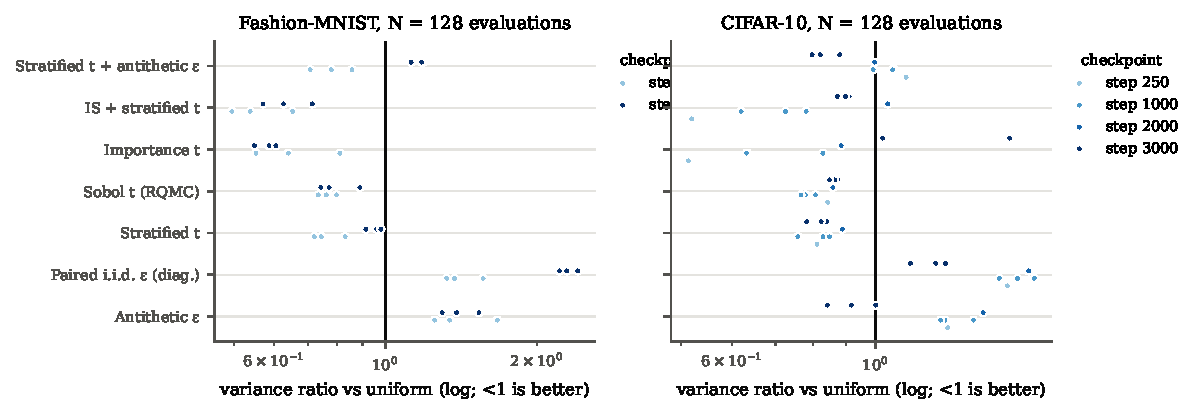
\includegraphics[width=\linewidth]{figures/var_ratio.pdf}
  \caption{\textbf{Gradient variance relative to uniform sampling at the same parameters and the same $N=128$.}
  Each dot is one (seed, checkpoint) probe with $R=48$ independent mini-batch gradients per estimator; colour
  shades mark the checkpoint. Values below 1 mean less variance. Stratified and Sobol timesteps are below 1
  everywhere. Antithetic noise is above 1 at most checkpoints, but always below its paired-i.i.d. control.
  Importance sampling moves from well below 1 to above 1 as training proceeds.}
  \label{fig:var}
\end{figure}

\paragraph{Gradient variance (Fig.~\ref{fig:var}, Table~\ref{tab:var}).}
\emph{Stratification works, but the gain is small.} On CIFAR-10, stratified timesteps give a variance ratio of
\StratVR\ at step 3000 (mean $\pm$ sd over 3 seeds) and \StratVRmin--\StratVRmax\ across all probes; the ratio is
below 1 in \StratVRbelow\ probes. Scrambled
Sobol timesteps behave the same (\SobolVR, \SobolVRbelow), as expected in one dimension (H1). The gain is
bounded by the between-timestep share of the variance, which is only \DecT\% (\S\ref{sec:where}).
\emph{Antithetic noise does not reduce variance at equal compute.} Its ratio is \AntiVR\ at step 3000 and
\AntiVRmin--\AntiVRmax\ over all probes (below 1 in \AntiVRbelow). The paired-i.i.d.\ control, which differs from
antithetic sampling only in the sign coupling, is far worse (\PairedVR), so the coupling works as intended.
What antithetic sampling cancels is roughly what it loses by sharing $(x_0,t)$ within a pair.
\emph{Importance sampling helps early and hurts late.} The loss-based proposal halves the variance at the first
probe (minimum ratio \ImpVRmin) but reaches \ImpVRmax\ by the end. Stratifying the IS uniforms stabilises it
(\ISSVR\ at step 3000; below 1 in \ISSVRbelow\ probes). On Fashion-MNIST, stratification, Sobol and
antithetic sampling behave the same way (\FStratVRmin--\FStratVRmax, \FSobolVRmin--\FSobolVRmax\ and
\FAntiVRmin--\FAntiVRmax). Importance sampling, however, reduces variance at every probe there
(\FImpVRmin--\FImpVRmax). Its late-training reversal is therefore specific to CIFAR-10 in our data, and the
800-step Fashion-MNIST runs may simply end before the proposal drifts. The unbiasedness check passes for every estimator
(\S\ref{sec:setup}).

\begin{table}[t]
  \centering\small
  \caption{\textbf{Gradient-variance ratio vs.\ uniform} ($\mathrm{tr}\,\mathrm{Cov}$, same $\theta$, $N=128$), mean $\pm$ sd over
  seeds. CIFAR-10 steps 250/2000 are seed 0 only, steps 1000/3000 have 3 seeds; Fashion-MNIST has 3 seeds.}
  \label{tab:var}
  \resizebox{\linewidth}{!}{\begin{tabular}{lrrrrrrrr}
\toprule
Estimator & fmnist @200 & fmnist @800 & cifar10 @250 & cifar10 @1000 & cifar10 @2000 & cifar10 @3000 & fmnist geo-mean [95\% CI] & cifar10 geo-mean [95\% CI] \\
\midrule
Antithetic $\epsilon$ & 1.42 $\pm$ 0.22 & 1.40 $\pm$ 0.12 & 1.29 & 1.32 $\pm$ 0.08 & 1.46 & 0.92 $\pm$ 0.08 & 1.41 [1.25, 1.58] & 1.16 [0.98, 1.38] \\
Paired i.i.d. $\epsilon$ (diag.) & 1.42 $\pm$ 0.13 & 2.31 $\pm$ 0.10 & 1.60 & 1.65 $\pm$ 0.10 & 1.72 & 1.22 $\pm$ 0.08 & 1.81 [1.35, 2.41] & 1.47 [1.28, 1.70] \\
Stratified t & 0.77 $\pm$ 0.06 & 0.95 $\pm$ 0.03 & 0.81 & 0.81 $\pm$ 0.05 & 0.89 & 0.82 $\pm$ 0.03 & 0.85 [0.74, 0.98] & 0.82 [0.79, 0.86] \\
Sobol t (RQMC) & 0.77 $\pm$ 0.03 & 0.80 $\pm$ 0.08 & 0.84 & 0.78 $\pm$ 0.02 & 0.86 & 0.86 $\pm$ 0.01 & 0.78 [0.73, 0.84] & 0.83 [0.80, 0.86] \\
Importance t & 0.67 $\pm$ 0.13 & 0.58 $\pm$ 0.03 & 0.51 & 0.70 $\pm$ 0.11 & 0.88 & 1.22 $\pm$ 0.34 & 0.62 [0.53, 0.72] & 0.84 [0.62, 1.14] \\
IS + stratified t & 0.56 $\pm$ 0.08 & 0.64 $\pm$ 0.07 & 0.52 & 0.71 $\pm$ 0.08 & 1.04 & 0.89 $\pm$ 0.02 & 0.60 [0.52, 0.69] & 0.78 [0.64, 0.94] \\
Stratified t + antithetic $\epsilon$ & 0.78 $\pm$ 0.07 & 1.16 $\pm$ 0.03 & 1.11 & 1.04 $\pm$ 0.04 & 1.00 & 0.83 $\pm$ 0.04 & 0.95 [0.75, 1.21] & 0.96 [0.86, 1.07] \\
\bottomrule
\end{tabular}
}
\end{table}

\begin{figure}[t]
  \centering
  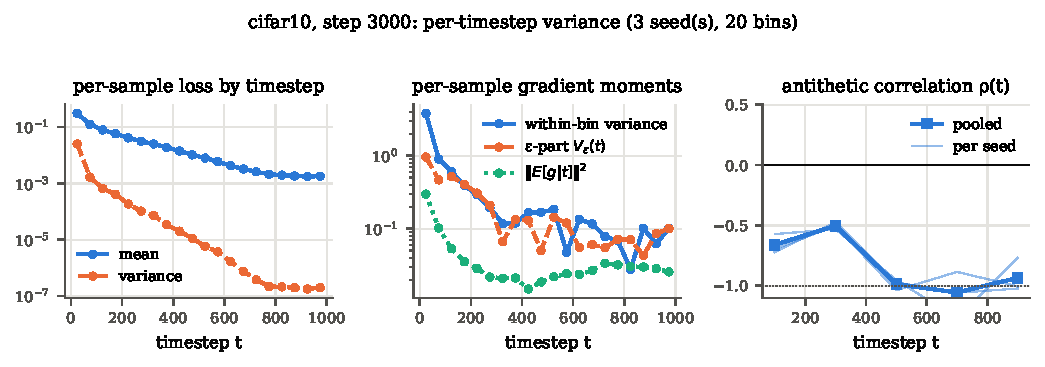
\includegraphics[width=\linewidth]{figures/per_t_cifar10.pdf}
  \caption{\textbf{Where the variance comes from (CIFAR-10, step 3000, 3 seeds).} Left: the per-sample loss and
  its variance fall by orders of magnitude from $t=0$ to $t=T$. Middle: the per-sample gradient moments vary far
  less. Right: the correlation between the gradients for $\epsilon$ and $-\epsilon$ (pooled over 4 bins and
  over seeds; thin lines are single seeds) is strongly negative at all $t$.}
  \label{fig:pert}
\end{figure}

\paragraph{Where the variance lives (Fig.~\ref{fig:pert}, Table~\ref{tab:decomp}).}
\label{sec:where}
On CIFAR-10 at step 3000, the per-sample gradient variance splits into \DecT\% between timesteps ($V_t$),
\DecX\% from the data given $t$ ($V_x$) and \DecE\% from the noise ($V_\epsilon$). This split explains the
results above. Stratifying $t$ can remove at most the 6\% between-timestep part plus some within-bin variation.
Antithetic noise attacks $V_\epsilon$ efficiently: $\rho=\Decrho$, close to the $-1$ of a locally affine network.
But by Eq.~\eqref{eq:anti} it helps only if $V_t+V_x<-\rho V_\epsilon$, and here
$V_t+V_x=\DecLHS$ while $-\rho V_\epsilon=\DecRHS$ (as fractions of the total). The condition fails, and it
fails more clearly on Fashion-MNIST, where the data term dominates ($V_x=\FDecX$\%, $\FDecLHS$ vs $\FDecRHS$).
The decomposition gets the ranking of the estimators right and predicts the absolute uniform variance to within
10\% on CIFAR-10. It overestimates the antithetic penalty at step 3000 (predicted \DecpAnti, measured \AntiVR).
For importance sampling, the loss-based proposal
$q\propto\sqrt{\mathbb E[\ell^2\mid t]}$ inherits the loss's $\approx$\LossRange$\times$ dynamic range across timesteps
(ratio of the largest to smallest bin), whereas $\sqrt{\mathbb E\|g\|^2\mid t}$ varies only $\approx$\GradRange$\times$. The
proposal therefore over-samples small $t$ and gives large weights to the rest. The gradient-optimal proposal
$q^\star$ would give a predicted ratio of \Decoracle\ on CIFAR-10 (\FDecoracle\ on Fashion-MNIST), the largest
reduction available from any timestep-only method here. This is a prediction, not a trained result.

\begin{table}[t]
  \centering\small
  \caption{\textbf{Law-of-total-variance decomposition and the variance ratios it predicts} (Eq.~\ref{eq:anti}),
  compared with the direct measurement at the same checkpoint. The last column is the absolute per-sample
  variance of the uniform estimator ($N\cdot\mathrm{tr}\,\mathrm{Cov}$), predicted and measured.}
  \label{tab:decomp}
  \resizebox{\linewidth}{!}{\begin{tabular}{lrrrrrr}
\toprule
 & stratified & antithetic & paired i.i.d. & strat+anti & oracle grad-IS & $N\,\mathrm{tr}\,\mathrm{Cov}$ (unif.) \\
\midrule
\multicolumn{7}{l}{\textit{Fashion-MNIST, step 800, 2 seed(s)}} \\
fractions $V_t / V_x / V_\epsilon$ & \multicolumn{6}{l}{5\% / 66\% / 30\%\quad pooled $\rho$ = -0.83 $\pm$ 0.14\quad $V_t+V_x$ = 0.70 vs $-\rho V_\epsilon$ = 0.25} \\
predicted ratio & 0.95 $\pm$ 0.00 & 1.46 $\pm$ 0.12 & 1.70 $\pm$ 0.04 & 1.36 $\pm$ 0.12 & 0.46 $\pm$ 0.05 & 2.170 $\pm$ 0.272 \\
measured ratio & 0.97 $\pm$ 0.01 & 1.41 $\pm$ 0.17 & 2.35 $\pm$ 0.08 & 1.16 $\pm$ 0.05 & -- & 1.642 $\pm$ 0.112 \\
\midrule
\multicolumn{7}{l}{\textit{CIFAR-10, step 3000, 3 seed(s)}} \\
fractions $V_t / V_x / V_\epsilon$ & \multicolumn{6}{l}{6\% / 44\% / 50\%\quad pooled $\rho$ = -0.71 $\pm$ 0.05\quad $V_t+V_x$ = 0.50 vs $-\rho V_\epsilon$ = 0.36} \\
predicted ratio & 0.94 $\pm$ 0.02 & 1.15 $\pm$ 0.05 & 1.50 $\pm$ 0.03 & 1.03 $\pm$ 0.05 & 0.62 $\pm$ 0.03 & 0.405 $\pm$ 0.011 \\
measured ratio & 0.82 $\pm$ 0.03 & 0.92 $\pm$ 0.08 & 1.22 $\pm$ 0.08 & 0.83 $\pm$ 0.04 & -- & 0.438 $\pm$ 0.012 \\
\bottomrule
\end{tabular}
}
\end{table}

\begin{table}[t]
  \centering\small
  \caption{\textbf{Training outcomes on CIFAR-10 at equal steps (3000) and equal evaluations per step.} Mean $\pm$ sd over
  seeds. $p$: two-sided Welch $t$-test against uniform (pre-registered). FID@1000/2000 are seed 0 only. The
  \ttt{strat\_anti} seed-2 run was trained without FID (PLAN A5), so its FID uses 2 seeds. ms/step excludes
  evaluation; T4 GPU, fp16.}
  \label{tab:main}
  \resizebox{\linewidth}{!}{\begin{tabular}{lrrrrrrrrr}
\toprule
Estimator & seeds & ms/step & overhead & held-out ($\times 10^{-3}$) & $p$ & FID@1000 & FID@2000 & FID@3000 & $p$ (FID) \\
\midrule
Uniform (baseline) & 3 & 90.8 & +0.0\% & 37.50 $\pm$ 0.18 & -- & 271.7 & 191.1 & 141.0 $\pm$ 5.7 & -- \\
Antithetic $\epsilon$ & 3 & 91.0 & +0.2\% & 37.75 $\pm$ 0.02 & 0.14 & 269.6 & 190.7 & 143.3 $\pm$ 3.0 & 0.58 \\
Stratified t & 3 & 90.4 & -0.5\% & 37.70 $\pm$ 0.22 & 0.29 & 270.2 & 190.5 & 140.0 $\pm$ 2.8 & 0.80 \\
Importance t & 3 & 92.2 & +1.5\% & 36.92 $\pm$ 0.32 & 0.07 & 269.1 & 184.8 & 135.3 $\pm$ 4.1 & 0.24 \\
Stratified t + antithetic $\epsilon$ & 3 & 89.4 & -1.6\% & 37.65 $\pm$ 0.19 & 0.37 & 271.7 & 189.3 & 141.2 $\pm$ 3.7 & 0.96 \\
\bottomrule
\end{tabular}
}
\end{table}

\begin{figure}[t]
  \centering
  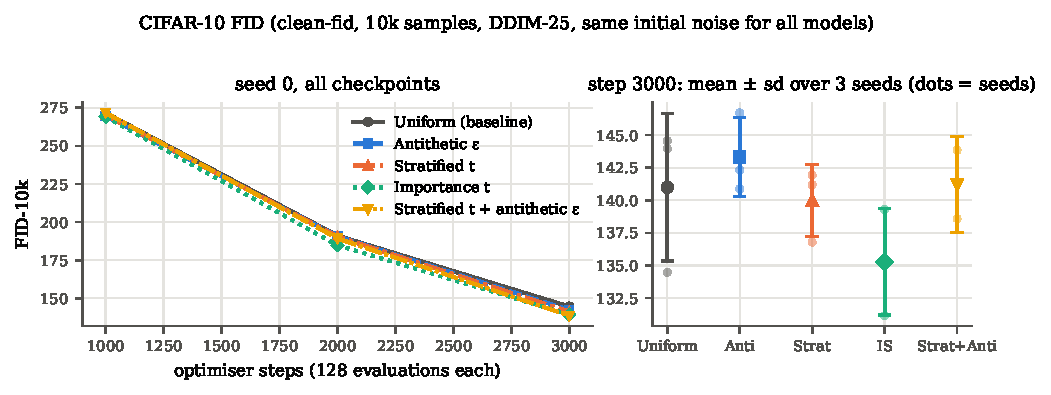
\includegraphics[width=\linewidth]{figures/fid_vs_steps_cifar10.pdf}
  \caption{\textbf{FID vs training steps (CIFAR-10).} Left: all checkpoints for seed 0. Right: step 3000, mean $\pm$ sd
  over seeds (dots are individual seeds). All estimators lie within one seed-to-seed standard deviation of uniform.}
  \label{fig:fid}
\end{figure}

\begin{figure}[t]
  \centering
  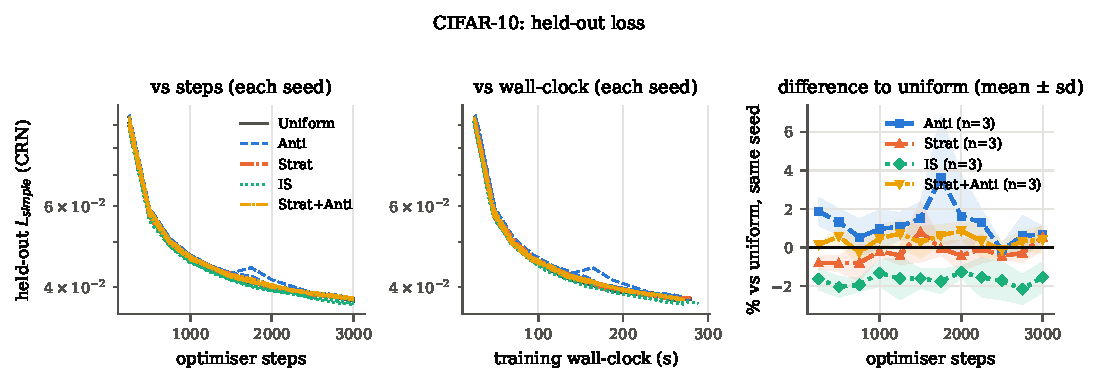
\includegraphics[width=\linewidth]{figures/loss_curves_cifar10.pdf}
  \caption{\textbf{Held-out loss (common random numbers) vs steps and vs wall-clock, CIFAR-10.} Right: relative difference
  to uniform for the same seed (same initialisation), mean $\pm$ sd. Importance sampling is consistently about
  1.5\% lower. The difference is not significant under the pre-registered test.}
  \label{fig:loss}
\end{figure}

\paragraph{Training outcomes (Table~\ref{tab:main}, Figs.~\ref{fig:fid}--\ref{fig:loss}).}
\emph{No estimator changes training outcomes significantly} (with 3 seeds, differences smaller than
$\approx$\MDEho\% in held-out loss or $\approx$\MDEfid\ FID are below the detection limit; \S\ref{sec:limitations}). At step 3000 the held-out loss
($\times10^{-3}$) is \UnifHO\ for uniform, \StratHO\ for stratified ($p=\StratpHO$), \AntiHO\ for antithetic
($p=\AntipHO$), \SAHO\ for stratified+antithetic ($p=\SApHO$) and \ImpHO\ for importance sampling
($p=\ImppHO$). FID-10k is \UnifFID\ (uniform), \StratFID, \AntiFID, \SAFID\ and \ImpFID\ respectively
(all $p\ge\ImppFID$). The 15--20\% variance reduction from stratification does not register in either metric.
Its effect on the held-out loss (\StratHOdiff\%) is far below the seed spread. Importance sampling is
best on both metrics despite \emph{higher} gradient variance late in training. In a secondary analysis that
pairs runs by seed (same initialisation and the same evaluation noise; not pre-registered), the differences
are \ImpHOpair\% in held-out loss ($p=\ImppHOpair$) and \ImpFIDpair FID ($p=\ImppFIDpair$). This is
suggestive but not significant. Gradient clipping was never active after warm-up in any arm (logged gradient
norms $\ll 1$), so clipping bias does not explain it. Two \emph{conjectures} we could not test within budget:
(a) the large early-training variance reduction (\ImpVRmin) gives IS a head start that persists; (b) because Adam
normalises each coordinate, re-allocating samples towards small $t$ changes the effective step size per
timestep, even though the gradient estimator is unbiased.
\emph{Overhead is negligible.} All estimators run at \UnifMS--\ImpMS\ ms/step (within $\pm$3\% of
uniform, inside timing noise), so loss vs wall-clock and loss vs steps are the same comparison.

\paragraph{Fashion-MNIST.} The CPU runs (\FSteps\ steps, 3 seeds) show the same pattern. Held-out loss
($\times10^{-3}$) is \FUnifHO\ (uniform), \FStratHO\ (stratified), \FAntiHO\ (antithetic), \FSAHO\ (strat+anti)
and \FImpHO\ (importance), with pre-registered $p$-values \FStratpHO, \FAntipHO, \FSApHO\ and \FImppHO. The
table is in Appendix~\ref{app:fmnist}.
